\chapter{Modified Fluid Closure of a Collisionless Plasma}\label{chap:kinbrag}
This chapter puts together the pieces of the previous chapters in order to approximate a collisionless plasma with a modified fluid closure. Limiting the pressure anisotropy as explained in Chapter~\ref{ssec:kinclosure} is compared to simulations without a pressure cap.

\section{Progress}
Currently, I am establishing if the limiter is doing what I expect. Figure~\ref{fig:eta2p} shows runs with resistivity $\eta=2*10^{-4}$ and the equivalent runs without the limiter in Figure~\ref{fig:eta2np}. The limiters seem to reduce the effect of resistivity and magnetic Prandtl number, since as seen in Figure~\ref{fig:eta3np} and Figure~\ref{fig:eta4np}, without the limiter there is wild variation. \\
\\
The viscous stress is also greatly affected by the limiter; without it, viscous stress dominated the total stress as seen in Figure~\ref{fig:visc}. With the limiter however, the viscous stress is negative (Figure~\ref{fig:viscnp}). Why is this?\\
\\
Looking at these trials in VisIt is also interesting: the linear evolution of the MRI seems to be quite different. Without the limiter I'm not sure I can find a linear growth stage; it just descends immediately into the channel mode (a double channel mode as compared to~\citetalias{BH1991c}) as shown in Figure~\ref{fig:t31}. With the limiter, the instability takes longer to develop. Figure~\ref{fig:t44} shows a good view of the linear development, with the uncapped version shown for comparison to already have descended into the turbulent regime.

\begin{figure}[h]
  \begin{center}  
    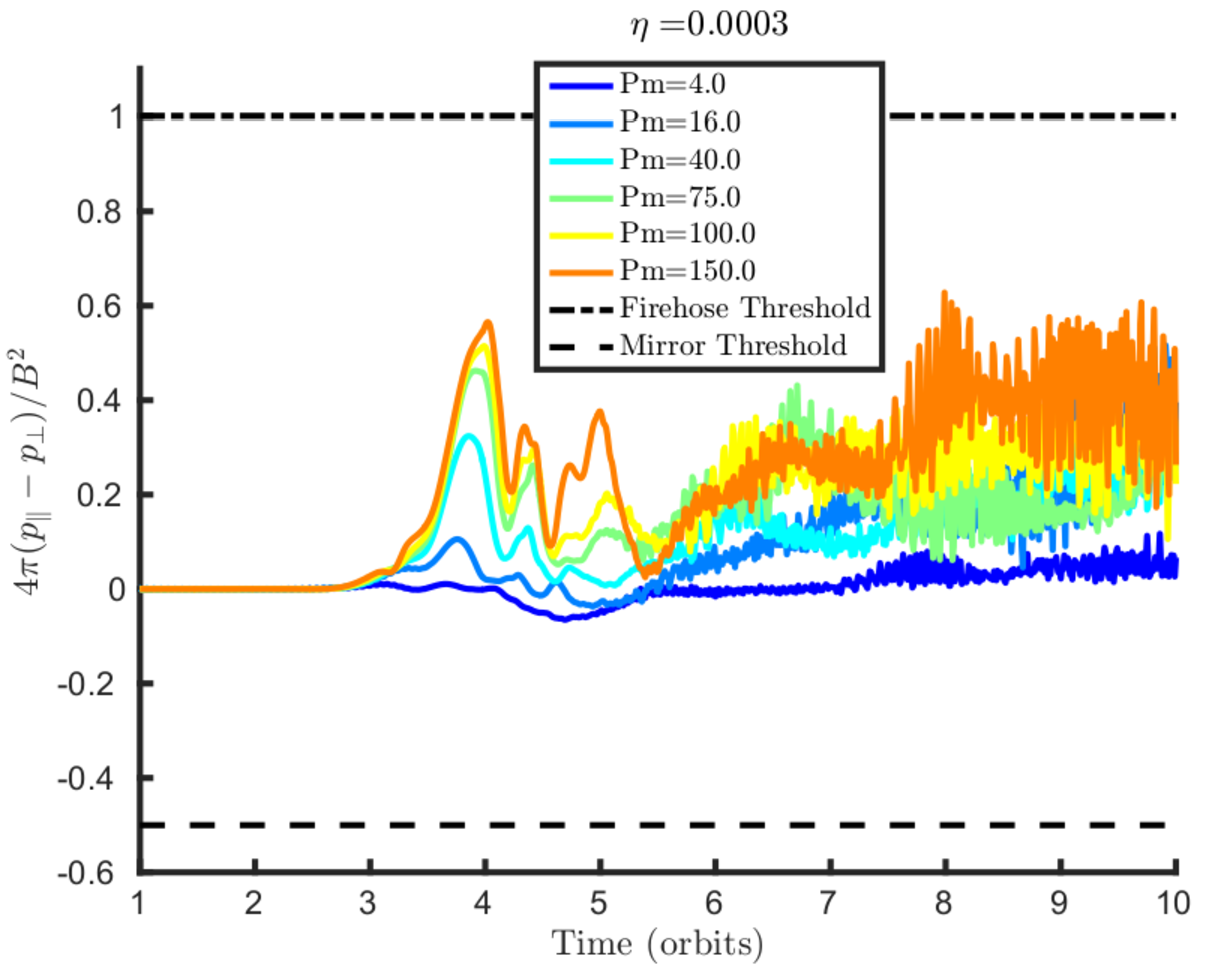
\includegraphics[width=.9\textwidth, angle=0.]{img/pLimiter-eta3-PmSel1_Sharma.pdf}
  \end{center}
  \caption{Simulations with $\eta=3e-3$, scanning $Pm$. Anisotropy is capped, but never actually gets close to either threshold.}
  \label{fig:eta2p}
\end{figure}

\begin{figure}[h]
  \begin{center}  
    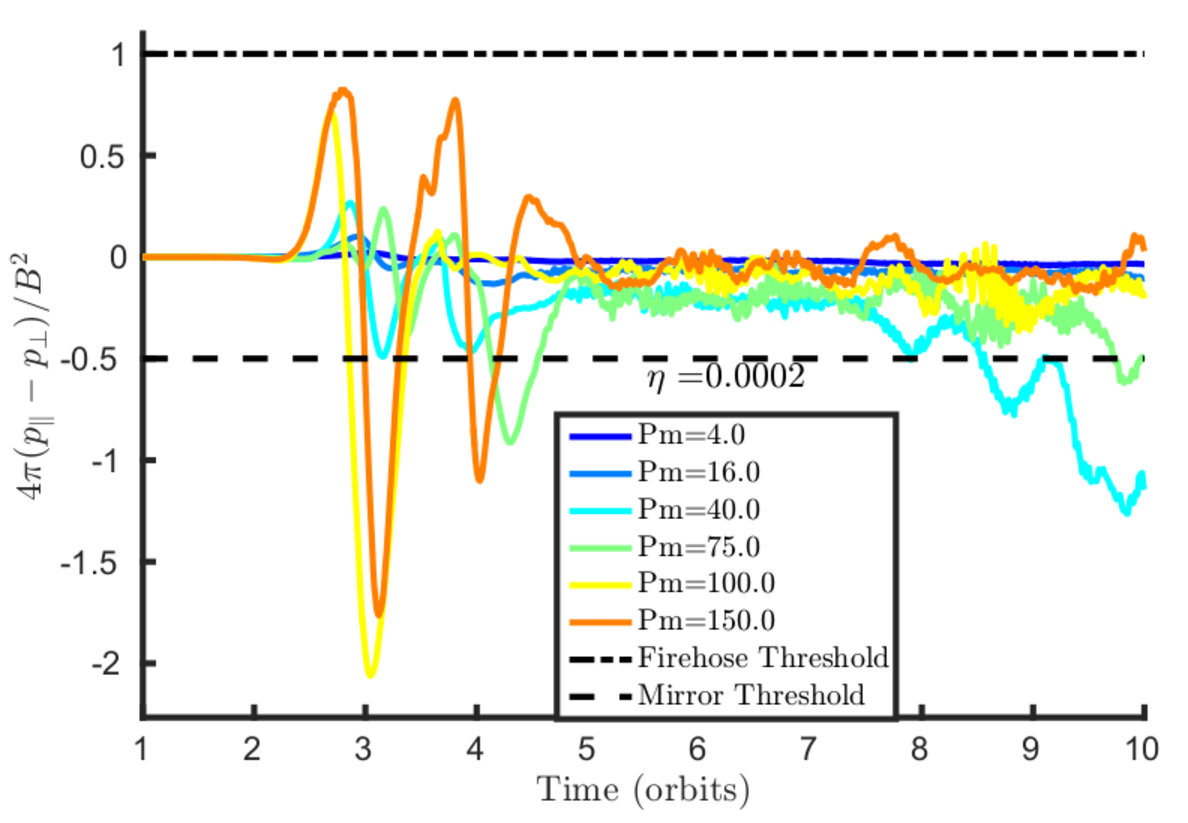
\includegraphics[width=.9\textwidth, angle=0.]{img/npLimiter-eta2-PmSel1_Sharma.pdf}
  \end{center}
  \caption{Simulations with $\eta=2e-3$, scanning $Pm$. Anisotropy is uncapped and greatly exceeds the mirror (but not the firehose) threshold. }
  \label{fig:eta2np}
\end{figure}


\begin{figure}[h]
  \begin{center}  
    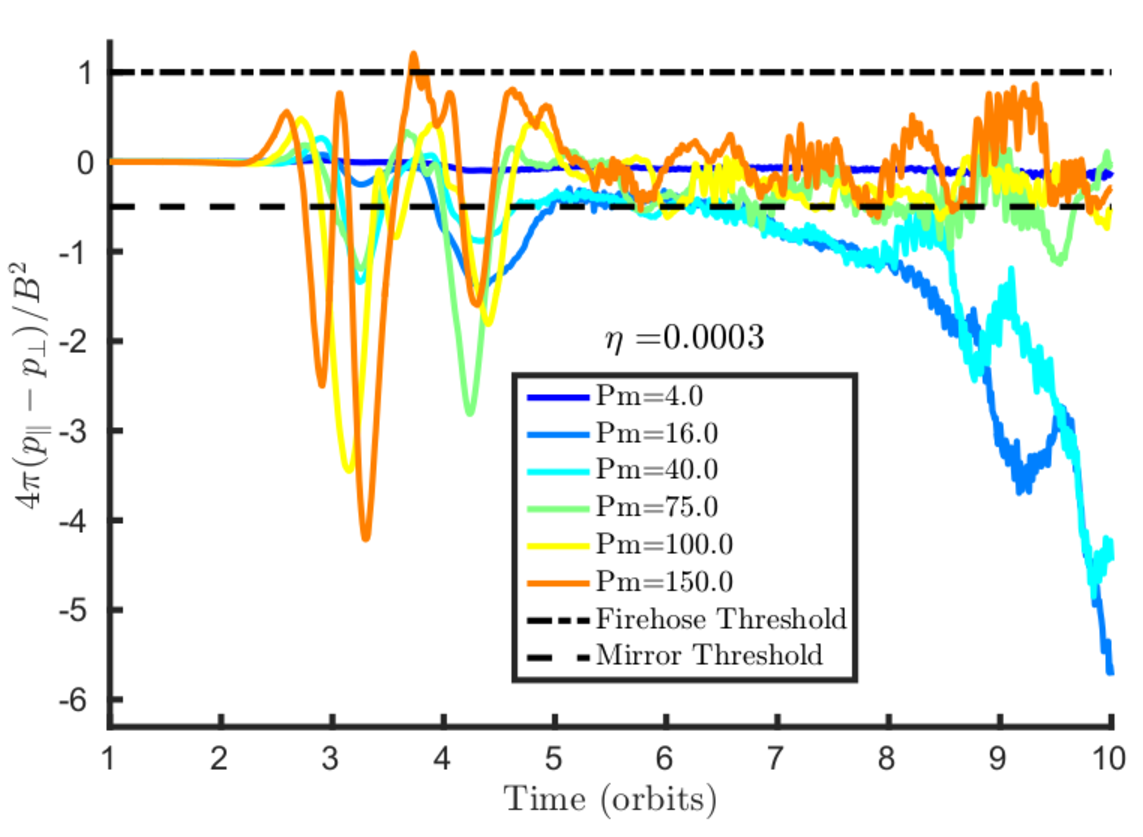
\includegraphics[width=.9\textwidth, angle=0.]{img/npLimiter-eta3-PmSel1_Sharma.pdf}
  \end{center}
  \caption{Simulations with $\eta=3e-3$, scanning $Pm$. Anisotropy is uncapped and exceeds both thresholds. Why do some $Pm$ start to grow instead of oscillating? }
  \label{fig:eta3np}
\end{figure}


\begin{figure}[h]
  \begin{center}  
    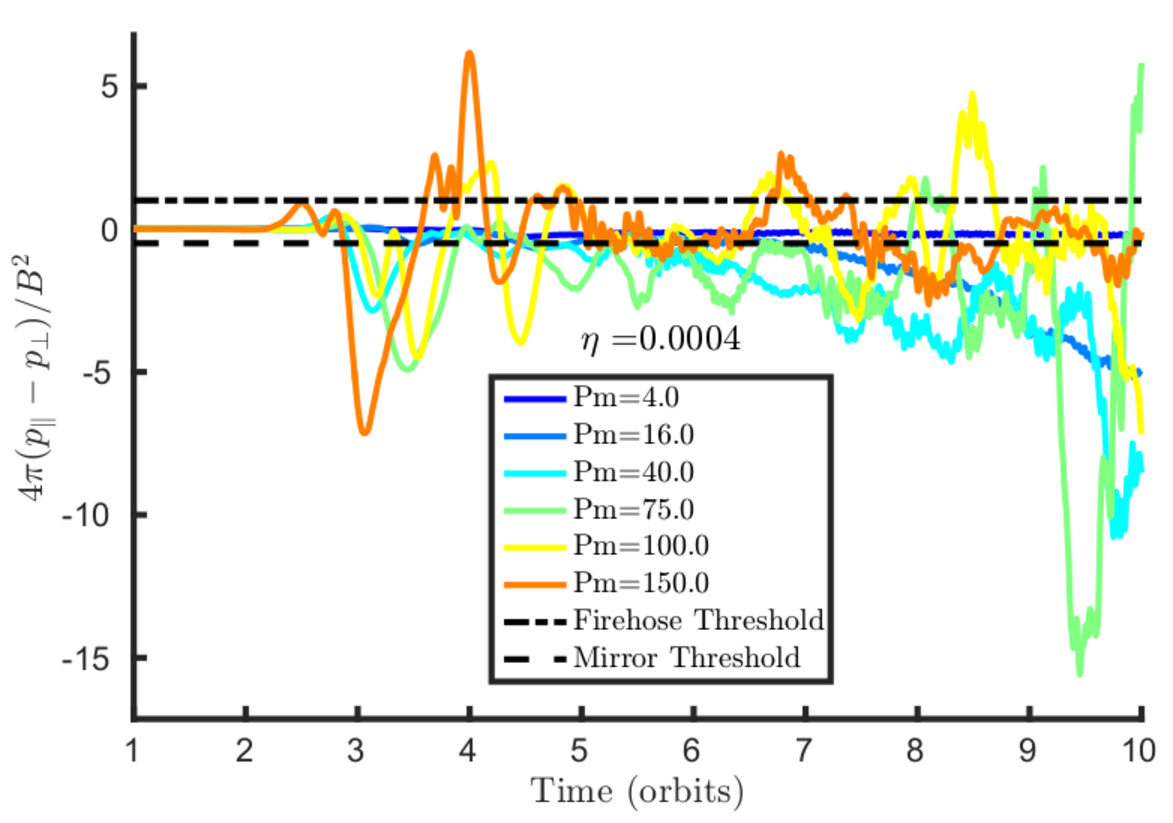
\includegraphics[width=.9\textwidth, angle=0.]{img/npLimiter-eta4-PmSel1_Sharma.pdf}
  \end{center}
  \caption{Simulations with $\eta=4e-3$, scanning $Pm$. Anisotropy is uncapped and mostly oscillatory...there is not a clear trend with increasing $Pm$. }
  \label{fig:eta4np}
\end{figure}


\begin{figure}[h]
  \begin{center}  
    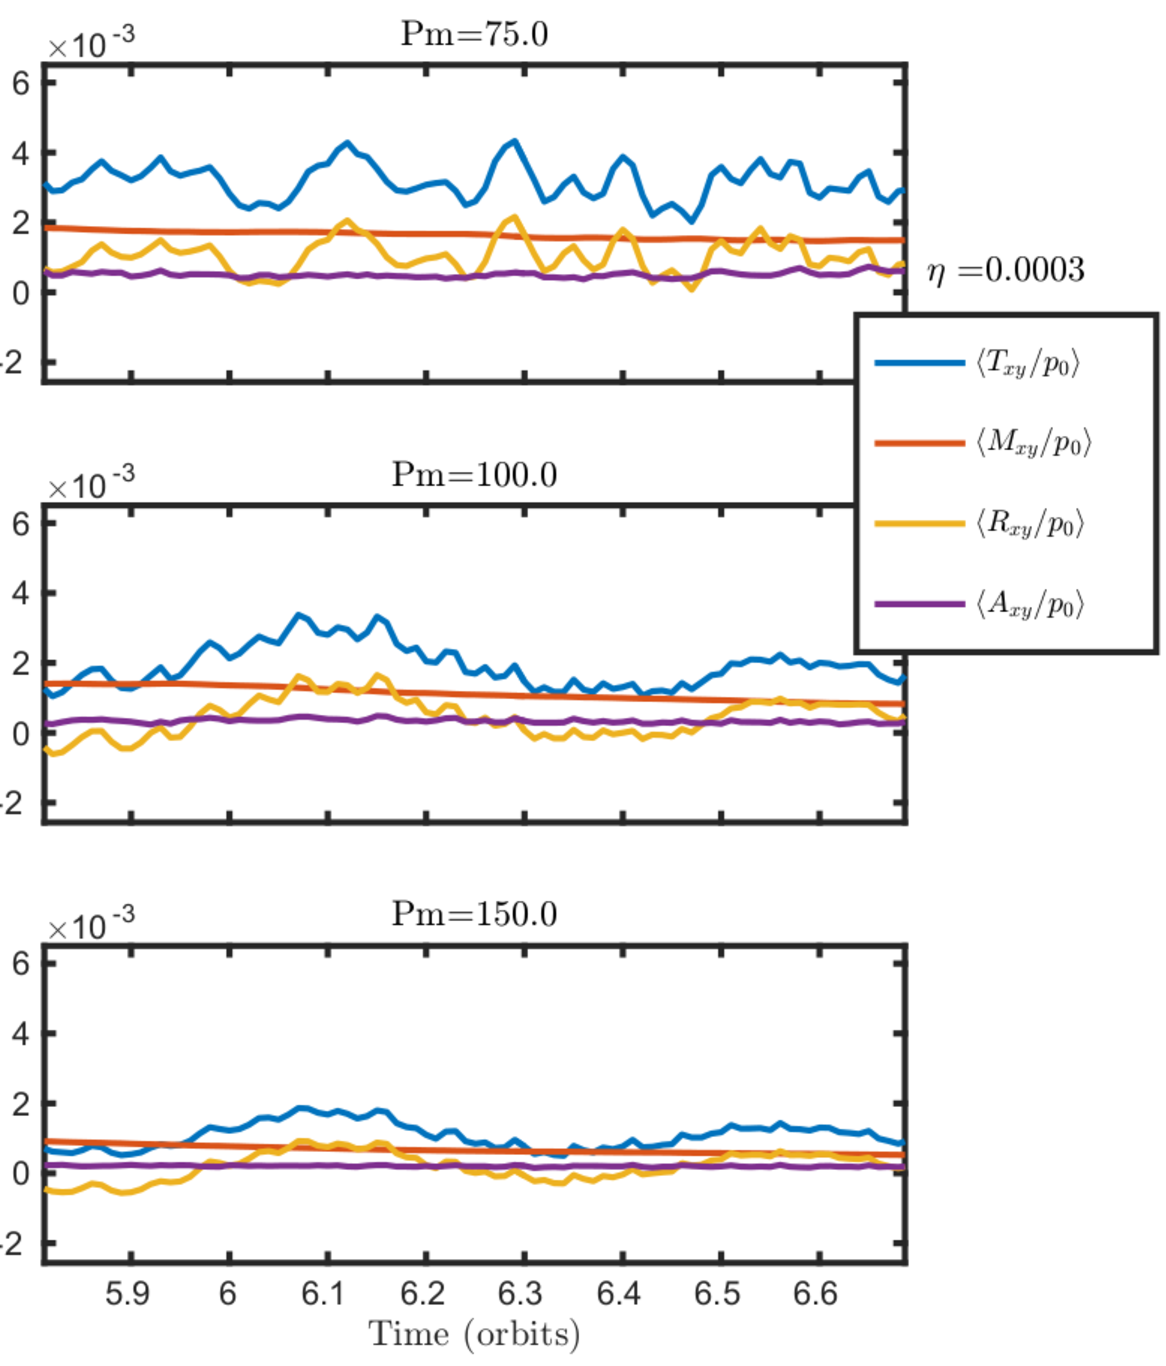
\includegraphics[width=.9\textwidth, angle=0.]{img/pLimiter-eta3-Pm11-13_StressesZoom_reversed.pdf}
  \end{center}
  \caption{Viscous stress, uncapped. The negative viscous stress is plotted. Why is the Reynolds stress comparable to the Maxwell stress? And why is it sinusoidal?}
  \label{fig:visc}
\end{figure}
\begin{figure}[h]
  \begin{center}  
    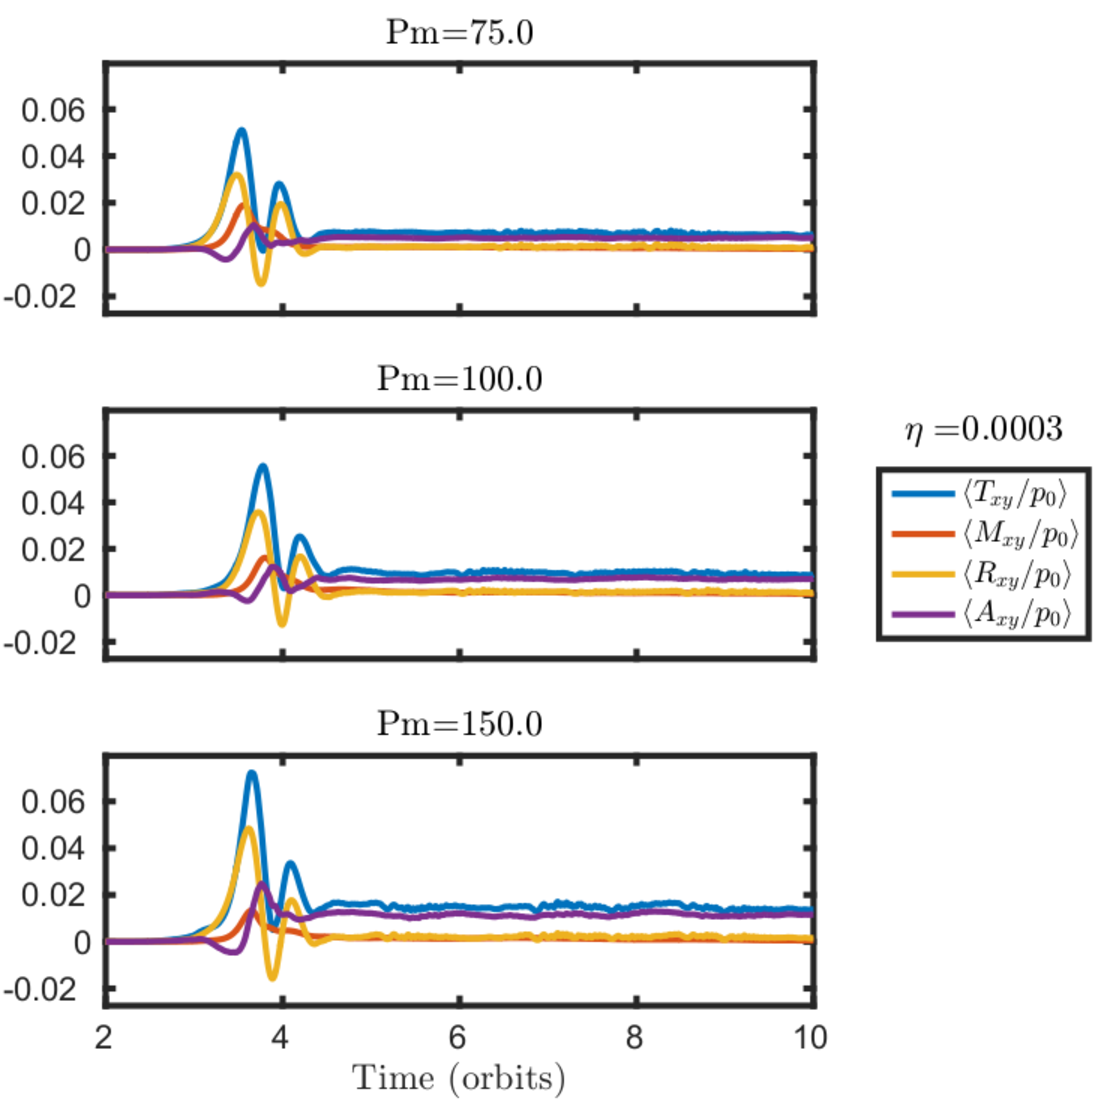
\includegraphics[width=.9\textwidth, angle=0.]{img/npLimiter-eta3-Pm11-13_StressesZoom.pdf}
  \end{center}
  \caption{Viscous stress, capped. This is more normal and shows that the viscous stress is greatly exceeding the Maxwell and Reynolds stresses.}
  \label{fig:viscnp}
\end{figure}


\begin{figure}[h]
  \begin{center}  
    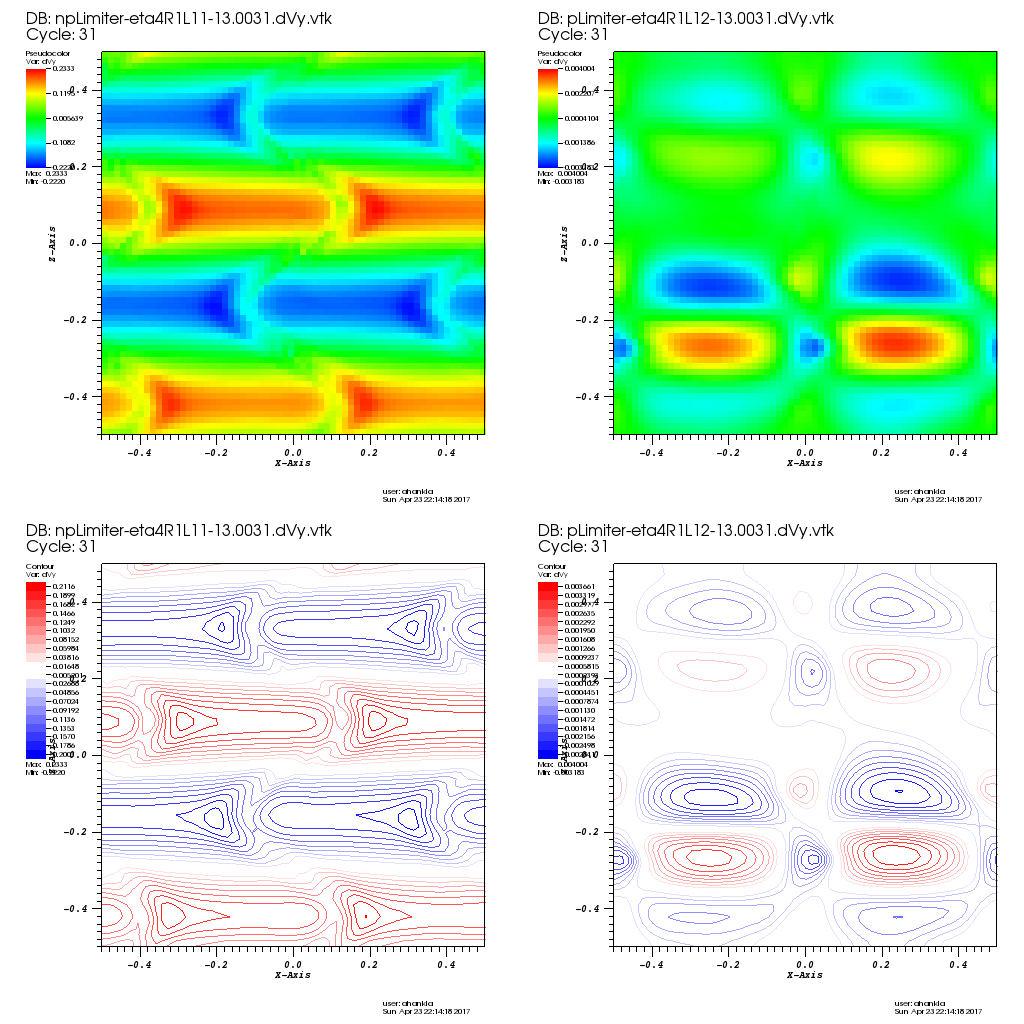
\includegraphics[width=.9\textwidth, angle=0.]{img/eta4_slice_dVy_t31.png}
  \end{center}
  \caption{Azimuthal angular momentum perturbations, t=3.1 orbits. Left column: uncapped. Right column: capped. $\eta=4e-4$. Is this the channel mode on the left, and linear growth on the right?}
  \label{fig:t31}
\end{figure}
\begin{figure}[h]
  \begin{center}  
    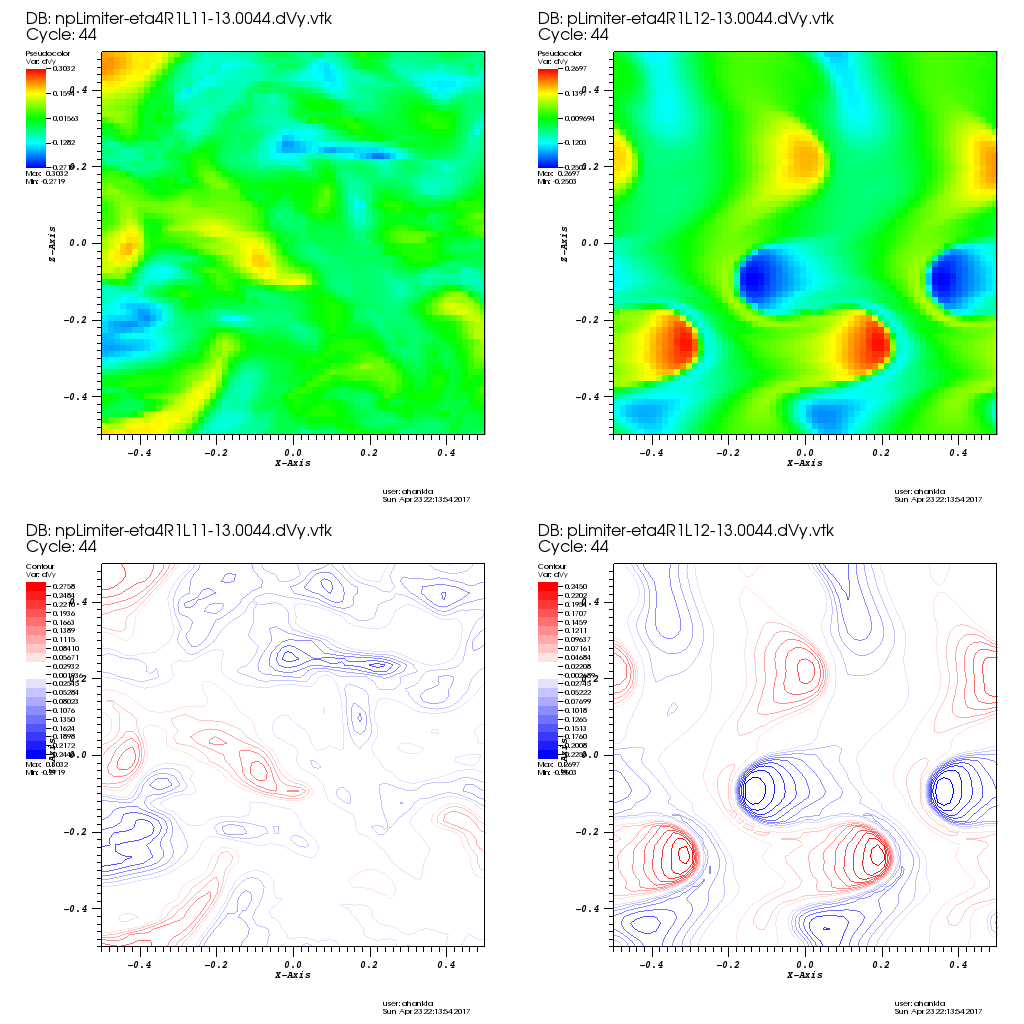
\includegraphics[width=.9\textwidth, angle=0.]{img/eta4_slice_dVy_t44.png}
  \end{center}
  \caption{Azimuthal angular momentum perturbations, t=4.4 orbits. Left column: uncapped. Right column: capped. $\eta=4e-4$. Is this the channel mode on the right?}
  \label{fig:t44}
\end{figure}

